

\section{The Standard Model from 1963 to 2012}\label{sec:THsm}


%\epigraph{Today I have done something which no theoretical physicist should ever do in his life: I have predicted something which shall never be detected experimentally!}{Wolfang Pauli to his friend Walter Baade}
\begin{flushright}
\begin{minipage}{.6\textwidth}
\begin{flushright}

\vskip5pt

\hrule 

\vskip7pt

{\it Today I have done something which no theoretical physicist should ever do in his life: I have predicted something which shall never be detected experimentally!}

\vskip5pt

\small{Wolfang Pauli to his friend Walter Baade}

\hrule

\vskip5pt


\end{flushright}
\end{minipage}
\end{flushright}


During the first half of the 20th century, many experimental 
discoveries were challenging particle physicists to find a 
coherent model to explain the existence of new particles and 
forces. A ``heavy electron'', the muon, was observed in 1936 
by C.%arl 
 Anderson and S.%eth 
 Neddermeyer in cosmic radiation, and later
observed in a cloud chamber experiment by %Jabez Curry 
J.C. Street and E. C. Stevenson~\cite{PhysRev.52.1003}. 
The neutrino, postulated in 1930 by %Wolfgang
W. Pauli\footnote{Pauli did not write a scientific
paper of his great intuition, which is only testified 
by a letter he sent to the 1930 Gauverein meeting in T\"ubingen,
famous also for his funny opening 
``{\it Dear Radioactive Ladies and Gentlemen,\dots}''. A copy
of the letter can be found in \url{http://tinyurl.com/cjgoubj}, 
and a nice history of the neutrino is in~\cite{2006physics...3106P}.}
to explain the shape of the electron 
spectrum in beta decay, was experimentally 
detected in 1956 by %Clyde L. 
C.L. Cowan and %Frederick 
F. Reines~\cite{1956Sci...124..103C}, and few years later a 
second neutrino type was discovered by %Leon M. 
L.M. Lederman, %Melvin 
M. Schwartz and %Jack 
J. Steinberger~\cite{1962PhRvL...9...36D}. 
By 1963 a huge number of new {\it mesons} and {\it baryons} 
were populating what was called the ``particle zoo'' 
until Murray Gell-Mann and George Zweig independently proposed 
a classification for all these new particles 
supposing that hadrons were made by smaller 
components~\cite{GellMann1964214,Zweig:352337}
(Figure~\ref{fig:eightfold} shows this particle classification referred to as 
``the eightfold way''\footnote{See e.g. \url{http://lccn.loc.gov/65013009}.}). 

\begin{figure}[htb]\begin{center}
	\subfigure[]{
  	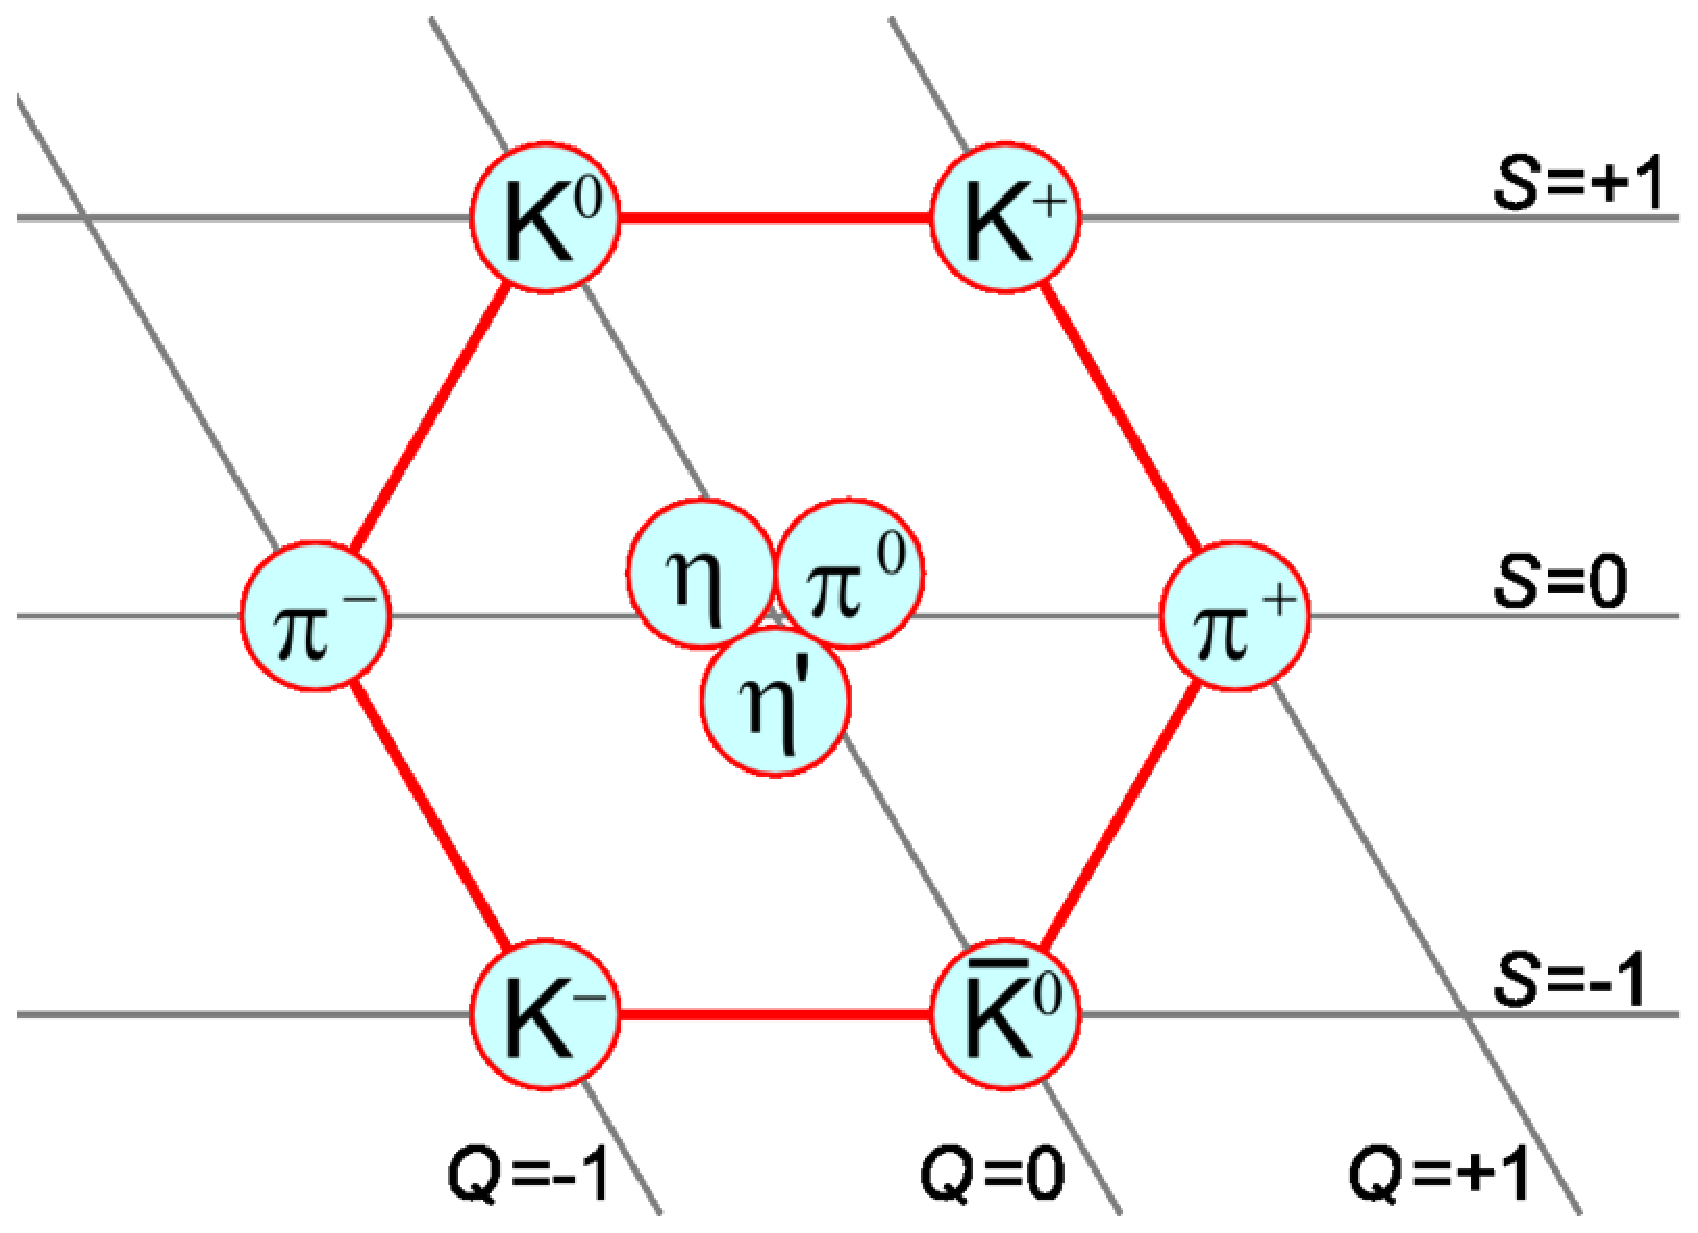
\includegraphics[width=0.4\textwidth]{theory/figures/mesons}}
	\subfigure[]{
  	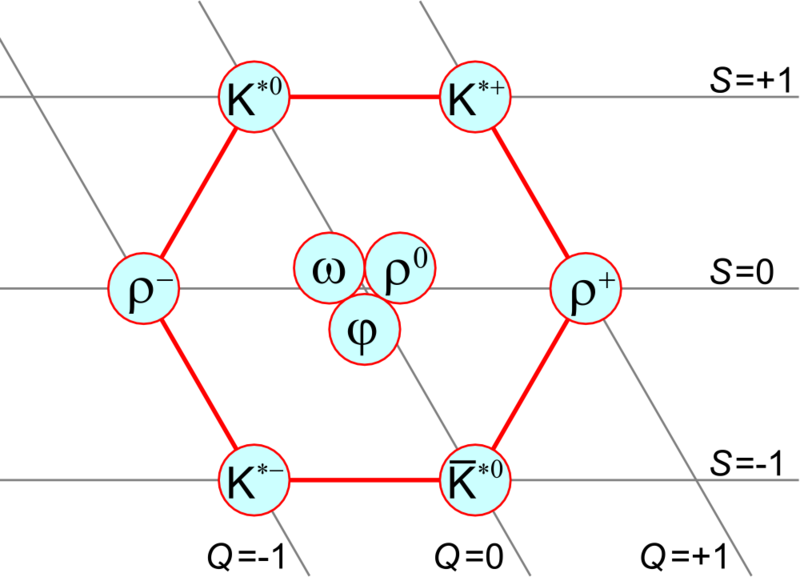
\includegraphics[width=0.4\textwidth]{theory/figures/mesons1}}
	\subfigure[]{
  	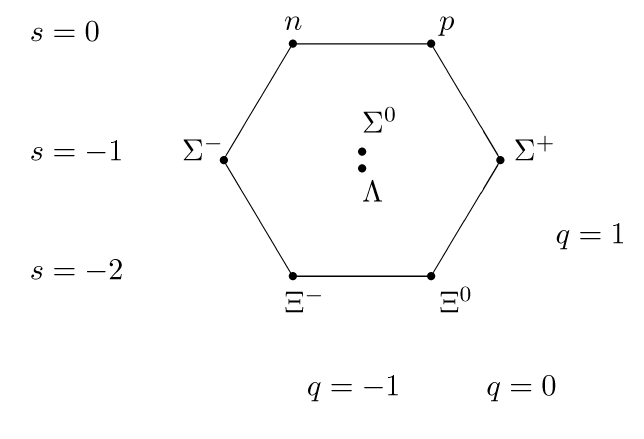
\includegraphics[width=0.4\textwidth]{theory/figures/Baryon_octet}}
	\subfigure[]{
  	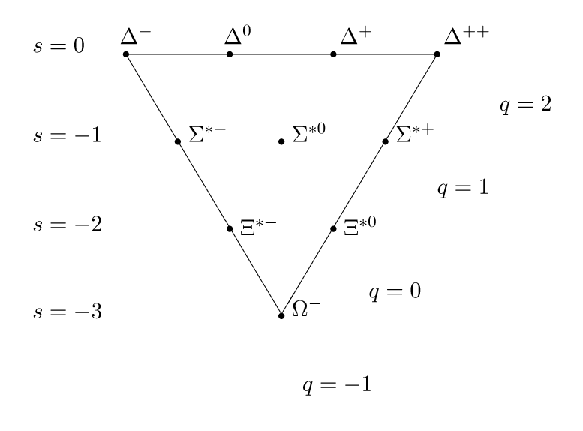
\includegraphics[width=0.4\textwidth]{theory/figures/Baryon_decuplet}}
	\caption{Gell-Mann's \textit{Eightfold Way} (proposed also independently 
          by Yuval Ne'eman) for (a) spin-0 meson octet, (b) spin-1 meson octet, 
          (c) spin-1/2 baryon octet (d) and spin-3/2 baryon decuplet, classified 
          through their electric charge $q$ and 
          strangeness $s$, % (from \cite{Nature74}). 
          but it is now understood that this structure is a 
          consequence of flavour symmetry.\label{fig:eightfold}}
\end{center}\end{figure}

It was the beginning of the {\it quark model}, a theory that had to 
wait for multiple experimental evidence before being accepted,
nevertheless it successfully predicted a new particle, the strangeness $s$=-3 
particle $\Omega^{-}$ of the spin-3/2 baryon decuplet of Figure~\ref{fig:eightfold},
discovered in 1964 at Brookhaven~\cite{PhysRevLett.12.204}. 
Even when in 1968 deep inelastic experiments at the Stanford 
Linear Accelerator Center (SLAC) found out evidence for a 
substructure in protons, physicists were reluctant to accept 
this point-like objects to be the quarks. Richard Feynman called 
them \textit{partons}, the term now used to identify quarks 
and antiquarks as well as gluons.

However, back then there was a tougher problem tormenting theoretical physicists. 
Quantum field theory was in fact apparently unsuitable for the description 
of the dynamics of particles interactions, since divergences appeared in the 
high energy domain. In 1954 Chen N. Yang and Robert Mills proposed a new gauge 
theory based on the principle of local gauge invariance i.e. the property of 
space-time regions of not being affected by a symmetry transformation performed 
locally in a different region. With the addition of a scalar field by Peter Higgs, 
Fran\c{c}ois Englert and Robert Brout and the implied modification of the vacuum 
structure (see Section \ref{sect:higgs} for more details), the Yang-Mills field 
became a very accurate description of the weak force interactions. Such model was 
consistently proposed in the 1960s by Abdus Salam, Sheldon Glashow and Steven 
Weinberg, but it suffered of a problem: as it was a perturbative theory, equations 
had to be expanded in a power series to be calculated but only the leading order 
term did not show ultraviolet divergences.

By the first years of the 1970s Martinus Veltman and Gerard't Hooft demonstrated 
renormalization for the theory, with the result that divergences could be 
cancelled and physical observables obtained with precisions higher than the 
leading order. 
The concept of \textit{renormalization group} was introduced and Yang-Mills theories were found to have a $\beta$-function (a function typical of gauge theories) generally negative. This was the discovery of \textit{asymptotic freedom}, a property that made Yang-Mills theory suitable also to describe strong interactions and that matched properly with the experimental effect named \textit{Bjorken scaling}\footnote{At SLAC it was observed during deep inelastic scattering experiments that strong interactions show a decrease of strenght at short distances (i.e. high momentum transfer) together with a scaling behaviour. A property is said to ``scale'' when it depends only by dimensionless kinematic quantities, such as a scattering angle or the ratio of the energy to a momentum transfer.}. 

At the same time, the three-quark model by Gell-Mann and Zweig was about to be expanded. In 1963 Nicola Cabibbo proposed the mixing of up, down and strange quark in order to explain the non-conservation of quark flavour in weak interactions as $\Lambda \rightarrow p^{+}\pi^{-}$ with $\Delta S$=1 and the empirical law $\Delta S = \Delta Q$ for strangeness changing processes. In 1970 Glashow, John Iliopoulos and Luciano Maiani (GIM) predicted a fourth quark, the charm, to account for the non observation of Strangeness Changing Neutral Current (SCNC) processes. Thus, the Cabibbo-GIM matrix $2\times 2$ parameterized by the Cabibbo angle $\theta_{C}$ described the quark mixing between these two families:
\begin{equation}\label{CabibboGIM}
V_{c} = {\setlength\arraycolsep{6pt}
\left( \begin{array}{cc}
\cos\theta_{C} & \sin\theta_{C}\\
-\sin\theta_{C}& \cos\theta_{C}
\end{array}
\right)} \quad .
\end{equation}
Furthermore, after the observation of CP violation events, Makoto Kobayashi and Toshihide Maskawa supposed the existence of two more quarks, the bottom and the top, thus increasing the number of quark flavours to six. This allowed the introduction in the new $3\times 3$ mixing matrix (the Cabibbo Kobayashi Maskawa CKM matrix) of, besides three angles, a complex phase that is responsible of CP violation. All this conjectures found an important confirmation in November 1974, known as the November Revolution maybe beacuse it was the beginning of a real trust in quark theory. Almost simultaneously at SLAC and at Brookhaven the charm quark was discovered in the bound state $c\bar c$, called $J$ meson by the Brookhaven team and $\psi$ by the SLAC one, so that in the end it was named $J/\psi$. Bottom quark was observed in 1977 at Fermilab, enhancing the belief in the top quark existence and in the six flavours theory.

The discovery of the tau lepton in 1978 and of the $W$ and $Z$ bosons in 1983 finally set the scene for the SM. Table \ref{tab:SM} shows the three generations of fermions, each of them having an antiparticle, and the three forces (three Yang-Mills fields) with their carriers composing the SM. A great achievement of the SM was the unification of electromagnetic and weak theories in the Electroweak Theory by Salam, Glashow and Weinberg. In fact, since at a scale of about 100 GeV the coupling constants converge, it is possible to describe them within the same mathematical model. Quantum ChromoDynamics (QCD) instead describes the strong interaction in terms of the color threefold charge and up to now is not known if also the strong coupling constant can become equal to the others at some high energy scale. However, a unified theory is strongly desired, as will be explained in Section \ref{sect:whyBSM}.
\begin{table}[htb]\centering\begin{tabular}{ccc|cc}
&\multicolumn{2}{c}{Leptons}&\multicolumn{2}{c}{Quarks} \\ 
& $q=-1$ & $q=0$ &$q=2/3$ &$q=-1/3$ \\ \hline
I & $e^{-}$ & $\nu_{e}$ & $u$ & $d$ \\
II & $\mu^{-}$ & $\nu_{\mu}$ & $c$ & $s$ \\
III & $\tau^{-}$ & $\nu_{\tau}$ & $t$ & $b$ \\\hline\hline
Force & Elm &\multicolumn{2}{c}{Weak}& Strong\\
Carrier & $\gamma$ & \multicolumn{2}{c}{$W^{\pm}$ \quad $Z$} & $g$\\\hline \hline
\end{tabular}\caption{Elementary particles and forces of the SM.}\label{tab:SM} \end{table}

Even if SM was born to be merely a stepping stone, it consolidated through years, standing all experimental tests sometimes with a precision greater than 0.1\%. Experiments carried out at LEP, thanks to the clean signals given by $e^{+}e^{-}$ collision events, allowed to obtain very high precision measurements of SM parameters. In particular experiments ALEPH, DELPHI, L3 and OPAL performed the measurements of the $Z$ boson mass with a precision of 0.0023\% that made it one of the most precisely known quantities within the SM\footnote{Note that the masses of the $W$ and $Z$ bosons are not predicted by the theory, but their ratio is (see Section \ref{sect:higgs}).}. Furthermore, measurements of its total decay width and of its partial decay widths for all processes with a visible final state (i.e. different from $\nu\bar\nu$) allowed to set the number of light neutrino flavours to three, confirming the three-generation SM and excluding the possibility for a fourth family of leptons with masses lower than half of $m_Z$.

The last discovery inside the SM has been the observation of the top quark in 1995 at the Fermilab's experiments CDF and D0. The mass of the top quark resulted consistent with the predicted constraints, thus confirming the SM as an accurate framework. There is a missing piece, though, that could invalidate all the previous beautiful confirmations, since the Higgs mechanism (Section \ref{sect:higgs}) is a cornerstone for the SM: a moderately light Higgs boson is in fact needed for the self-consistency of the overall fit of data. At present a preferred value of 80 GeV for the Higgs mass is predicted from precision measurements, although the lower limit from direct searches is 114 GeV with an upper limit of 144 GeV at 95\% C.L. \cite{Renton} (Figure \ref{higgsMass}). However, there are almost no doubts about the overall consistency of the SM. Figure \ref{higgsMass} shows a comparison between high precision measurements and values obtained from the fit \cite{Renton}.


